\section{Experiment 9E: causal audit of the Local advantage}
\label{sec:experiment9e}

\paragraph{Question.}
The preceding experiments consistently show that a separately fitted Local
controller gives the lowest tracking error. Experiment 9E asks whether this is
caused by genuine vehicle-specific information, an identification artifact that
compensates the nonlinear plant, an inappropriate parameter metric, or favorable
calibration--deployment matching. This is a diagnostic experiment and has no
positive-result gate: its purpose is to determine what must be redesigned before
claiming an accuracy benefit from information sharing.

Ten fresh fleets (seeds 146--155) each contain 30 test vehicles. Every vehicle
receives the frozen 9D adaptive calibration protocol and stops after 1.75~s. Five
controllers isolate distinct effects: Local uses the fitted client ratios;
Exact-individual uses its true simulator ratios; Swap-within-family uses the
Local fit of the next vehicle in the same true family; Exact-family uses the
geometric mean of the true ratios within each family; and Global-exact uses the
population geometric mean. Thus Exact-family is a deliberately stronger sharing
reference than a learned or federated family estimate: it has neither clustering
nor estimation error. An Exact-deployment reference is additionally recomputed
after drift and is not a deployable method.

All fixed controllers are evaluated on the nominal plant and after two common
post-calibration changes: a 10\% loss of both axle stiffnesses and a load shift
that raises mass by 10\% and yaw inertia by 12\%. The same drift is applied to
every method. Besides closed-loop tracking, the audit records unweighted
log-parameter error, scheduled-gain error relative to Exact-individual, and
normalized held-out nonlinear prediction error.

\begin{table}[htbp]
\centering
\caption{Experiment 9E tracking RMSE on ten fresh fleets. Parentheses report
change relative to Local in the same condition.}
\label{tab:experiment9e-results}
\begin{tabular}{lrrr}
\toprule
Method & Nominal & Tire fade & Load shift\\
\midrule
Exact-deployment & 0.006702 ($-3.89\%$) & 0.006868 ($-10.34\%$) & 0.006995 ($-9.48\%$)\\
Exact-individual & 0.006702 ($-3.89\%$) & 0.007348 ($-4.07\%$) & 0.007425 ($-3.91\%$)\\
Local & 0.006974 & 0.007660 & 0.007728\\
Exact-family & 0.007521 ($+7.85\%$) & 0.008286 ($+8.18\%$) & 0.008339 ($+7.91\%$)\\
Swap-within-family & 0.008569 ($+22.88\%$) & 0.009448 ($+23.33\%$) & 0.009477 ($+22.64\%$)\\
Global-exact & 0.011638 ($+66.89\%$) & 0.012814 ($+67.28\%$) & 0.012795 ($+65.58\%$)\\
\bottomrule
\end{tabular}
\end{table}

\begin{figure}[htbp]
\centering
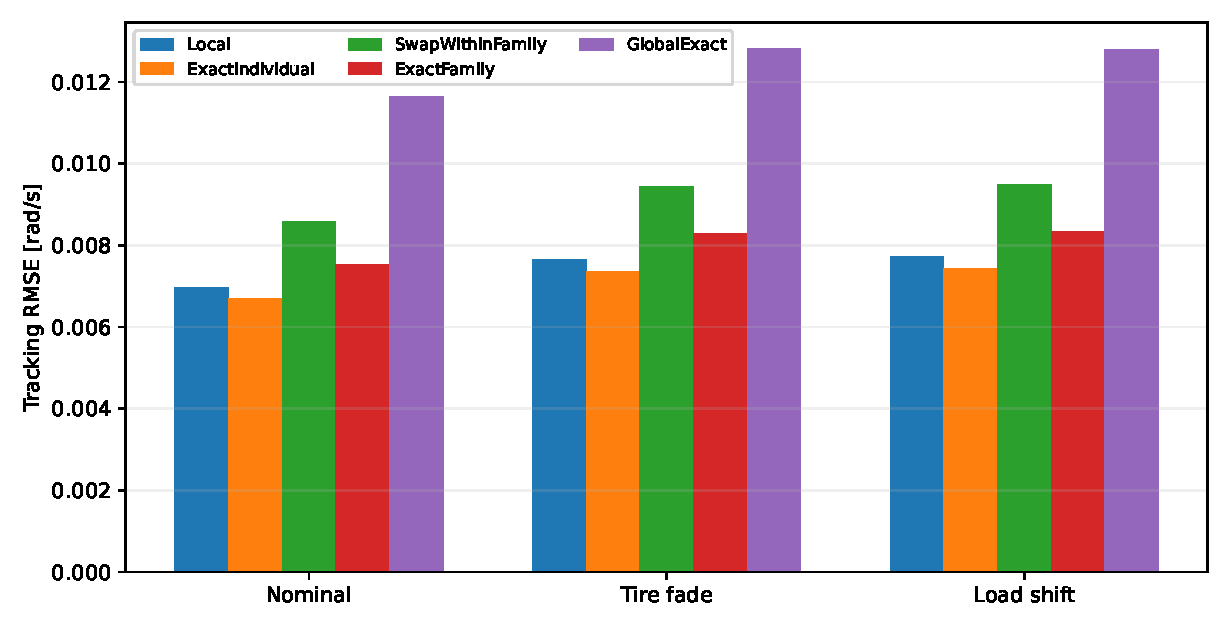
\includegraphics[width=0.82\linewidth]{../results/figures/experiment_9e_local_advantage_audit.pdf}
\caption{Local-advantage decomposition under matched and shifted deployment.}
\label{fig:experiment9e}
\end{figure}

\paragraph{Attribution.}
Exact-individual improves nominal tracking by 3.89\% over Local. Consequently,
the Local fit is not winning by learning a beneficial but physically incorrect
surrogate for the nonlinear plant; finite-data estimation still leaves a small
recoverable loss. In contrast, substituting another correctly classified family
member worsens Local by 22.88\%. Even Exact-family, which knows the true family
and its exact mean ratios, is 7.85\% worse. Most of the remaining Local advantage
therefore comes from real within-family specialization, not federated
optimization, clustering, or privacy error.

The diagnostic measures explain why scalar parameter error was previously
misleading. Across clients, Local log-parameter error has Spearman correlation
$\rho=0.029$ with tracking, whereas scheduled-gain error has $\rho=0.216$ and
held-out nonlinear prediction error has $\rho=0.325$. For the shared
comparators the control-aligned measures are much more predictive: Exact-family
gain and prediction correlations are 0.757 and 0.708, and Global-exact values
are 0.873 and 0.937. Parameter distance treats all three identified ratios as
equally important even though their closed-loop consequences differ.

The two deployment shifts increase absolute errors but preserve the ordering
and nearly the same relative gaps. Fixed Local remains about 4\% behind the
drift-unaware Exact-individual controller and approximately 8\% ahead of
Exact-family. The tested drift therefore does not provide evidence for replacing
Local with a shared controller on robustness grounds. All 300 fits converge and
all 16,200 nonlinear closed-loop evaluations remain feasible.

\paragraph{Decision.}
Experiment 9E rejects two tempting repairs: improving family discovery alone
cannot erase the exact-family gap, and changing only the reporting metric cannot
erase the closed-loop gap. It also shows why deliberately shortening or
degrading Local data would move the goalposts rather than solve the scientific
problem.

The defensible next model is a shared family backbone plus a low-dimensional
local, control-relevant residual. Federation should learn the common scheduled
dynamics or controller basis, while each vehicle retains only the few local
coordinates that materially change its gain schedule. The resulting comparison
should be against full Local using three separate axes: closed-loop quality,
local calibration burden, and deployed degrees of freedom. Identification and
aggregation should select residual directions using gain sensitivity or
closed-loop validation, not isotropic log-parameter distance. A useful next
experiment must therefore ask how many local residual coordinates are required
to close the 7.85\% exact-family gap; it should not ask whether a single shared
family model can outperform a correctly specialized Local controller.

\paragraph{Reproducibility.}
The protocol is frozen in \path{code/config/experiment_9e.json} and implemented
in \path{code/experiments/experiment_9e_local_advantage_audit.py}. Seed-level
results, diagnostic correlations, comparisons, provenance hashes, and the
figure source data are retained under \path{results/tables}.
